\documentclass[12pt,oneside,a4paper,parskip]{scrbook}
\usepackage[utf8]{inputenc}
\usepackage{csquotes}
%\usepackage[ngerman]{babel}
\usepackage{floatflt}
\usepackage{subfigure}
\usepackage[pdftex]{graphicx}
\usepackage[hidelinks]{hyperref}
\usepackage{color}
\usepackage{amssymb}
\usepackage{textcomp}
\usepackage{nicefrac}
\usepackage{scrhack}
\usepackage{pdfpages}
\usepackage{float}
\usepackage{pdflscape}
\usepackage{subfigure}
\usepackage{pdfpages}
\usepackage[verbose]{placeins}
\usepackage[nouppercase,headsepline,plainfootsepline]{scrlayer-scrpage}
\usepackage{listings}
\usepackage{xcolor}
\usepackage{color}
\usepackage{caption}
\usepackage{subfigure}
\usepackage{epstopdf}
\usepackage{longtable}
\usepackage{setspace}
\usepackage{booktabs}
\usepackage{nameref}
\usepackage[
backend=biber,
style=apa,
citestyle=authoryear-comp
]{biblatex}

\bibliography{bibliography}


%% Schauen ob die Reihenfolge passt

%%%%%%%%%%%%%%%%%%%
%% definitions
%%%%%%%%%%%%%%%%%%%
\def\BaAuthor{Achim Winter}
\def\BaAuthorStudyProgram{Computer Science}
\def\BaType{Bachelor thesis} %% passt das so?
\def\BaTitle{Operating a Smartphone as a Hardware Security Module}
\def\BaSupervisorOne{Prof.\ Dr.\ Junker-Schilling}
\def\BaSupervisorTwo{Prof.\ Dr.\ Huffstadt}
\def\BaDeadline{\today}

\ifdefined\iswithfullname
  \def\ShowBaAuthor{\BaAuthor}
\else
  \def\ShowBaAuthor{N.~N.}
\fi

\hypersetup{
pdfauthor={\ShowBaAuthor},
pdftitle={\BaTitle},
pdfsubject={Subject},
pdfkeywords={Keywords}
}

%%%%%%%%%%%%%%%%%%%
%% configs to include
%%%%%%%%%%%%%%%%%%%
\colorlet{punct}{red!60!black}
\definecolor{background}{HTML}{EEEEEE}
\definecolor{delim}{RGB}{20,105,176}
\colorlet{numb}{magenta!60!black}

\definecolor{gray}{rgb}{0.4,0.4,0.4}
\definecolor{darkblue}{rgb}{0.0,0.0,0.6}
\definecolor{cyan}{rgb}{0.0,0.6,0.6}

\definecolor{pblue}{rgb}{0.13,0.13,1}
\definecolor{pgreen}{rgb}{0,0.5,0}
\definecolor{pred}{rgb}{0.9,0,0}
\definecolor{pgrey}{rgb}{0.46,0.45,0.48}

\lstset{
  basicstyle=\ttfamily,
  columns=fullflexible,
  showstringspaces=false,
  commentstyle=\color{gray}\upshape
  linewidth=\textwidth
}

\lstdefinelanguage{json}{
    basicstyle=\normalfont\ttfamily,
    numbers=left,
    numberstyle=\scriptsize,
    stepnumber=1,
    numbersep=8pt,
    showstringspaces=false,
    breaklines=true,
    backgroundcolor=\color{background},
    literate=
     *{0}{{{\color{numb}0}}}{1}
      {1}{{{\color{numb}1}}}{1}
      {2}{{{\color{numb}2}}}{1}
      {3}{{{\color{numb}3}}}{1}
      {4}{{{\color{numb}4}}}{1}
      {5}{{{\color{numb}5}}}{1}
      {6}{{{\color{numb}6}}}{1}
      {7}{{{\color{numb}7}}}{1}
      {8}{{{\color{numb}8}}}{1}
      {9}{{{\color{numb}9}}}{1}
      {:}{{{\color{punct}{:}}}}{1}
      {,}{{{\color{punct}{,}}}}{1}
      {\{}{{{\color{delim}{\{}}}}{1}
      {\}}{{{\color{delim}{\}}}}}{1}
      {[}{{{\color{delim}{[}}}}{1}
      {]}{{{\color{delim}{]}}}}{1},
}

\lstset{language=xml,
  morestring=[b]",
  morestring=[s]{>}{<},
  morecomment=[s]{<?}{?>},
  stringstyle=\color{black},
  numbers=left,
  numberstyle=\scriptsize,
  stepnumber=1,
  numbersep=8pt,
  identifierstyle=\color{darkblue},
  keywordstyle=\color{cyan},
  backgroundcolor=\color{background},
  morekeywords={xmlns,version,type}% list your attributes here
}

\lstset{language=Java,
  showspaces=false,
  showtabs=false,
  tabsize=4,
  breaklines=true,
  keepspaces=true,
  numbers=left,
  numberstyle=\scriptsize,
  stepnumber=1,
  numbersep=8pt,
  showstringspaces=false,
  breakatwhitespace=true,
  commentstyle=\color{pgreen},
  keywordstyle=\color{pblue},
  stringstyle=\color{pred},
  basicstyle=\ttfamily,
  backgroundcolor=\color{background},
%  moredelim=[il][\textcolor{pgrey}]{$$},
%  moredelim=[is][\textcolor{pgrey}]{\%\%}{\%\%}
}

\newcommand*{\forcetwosidetitle}[1][1]{%
 \begingroup
   \cleardoubleoddpage
   \KOMAoptions{titlepage=true}% useful e.g. for scrartcl
   \csname @twosidetrue\endcsname
   \maketitle[{#1}]
 \endgroup
}


\begin{document}


%%%%%%%%%%%%%%%%%%%
%% Titelseite
%%%%%%%%%%%%%%%%%%%


\frontmatter
\titlehead{%  {\centering Seitenkopf}
  {University of applied Sciences W\"{u}rzburg-Schweinfurt\\
   Faculty of Computer Science und Business Informatics}}
\subject{\BaType}
\title{\BaTitle\\[15mm]}
\subtitle{\normalsize{submitted to the University of Applied Sciences W\"{u}rzburg-Schweinfurt in the Faculty of \BaAuthorStudyProgram}}
\author{\ShowBaAuthor}
\date{\normalsize{Submitted on: \BaDeadline}}
\publishers{
  \normalsize{First Supervisor: \BaSupervisorOne}\\
  \normalsize{Second Supervisor: \BaSupervisorTwo}\\
}
%\lowertitleback{
%\centering
\includegraphics[width=4cm]{barcode_default}

%}
\forcetwosidetitle


%%%%%%%%%%%%%%%%%%%
%% abstract
%%%%%%%%%%%%%%%%%%%

\section*{Summary}
TODO

\section*{Abstract}

TODO

\newpage
\chapter*{Acknowledgment}

I would like to thank Prof. Dr. Junker-Schilling for his helpful support. The seminars and the discussions with the other students helped me a lot to stay on schedule and make the work what it is now. My further thanks go to Prof. Dr. Huffstadt for the second correction. 

I would also like to thank Francis Pouatcha and Steffen Blümm for their support from adorsys. The discussions always brought new ideas on how the work can be further improved. Thank you very much for that.

I would also like to thank my proofreaders and my family. Thanks to you too, the work has become what it is today.

%%%%%%%%%%%%%%%%%%%
%% Inhaltsverzeichnis
%%%%%%%%%%%%%%%%%%%
\tableofcontents



%%%%%%%%%%%%%%%%%%%
%% Main part of the thesis
%%%%%%%%%%%%%%%%%%%
\mainmatter

\chapter{Introduction}\label{ch:intro}

The two main fields of cryptography in computer systems can be divided between symmetric-key cryptography and public-key cryptography. Symmetric-key utilizes the same key for the sender and the receiver, which was the first form of encryption and also secure and easy to understand. If this is done by close relatives this may be possible, but exchanging this key to every website when browsing through the internet is impractical. Not only because it is physically nearly impossible, but also because the amount of keys one would have to store securely would be growing by the square of number of communication partners.
% Maybe a picture for symmetric encryption
To avoid this kind of key management, Whitfield Diffie and Martin Hellman published a system in 1976 known as the public-key cryptography. With this system it is possible to generate an encryption key over an insecure network such as the Internet in order to secure subsequent communication. However, the real encryption key is never transferred to the opposing communication partner. In fact the real encryption key is being calculated by using public and private keys, which have a mathematical relation to each other. Each communication partner has to create a pair of his own private and public key. While the public key can be exposed to the Internet, the private key has to remain secret. 
By using both key pairs, a common shared key can be calculated which then can be used for the encryption. This system relies on the computational complexity, such as prime factorization, which is hard to do with big numbers. 
%[Was ist der Diffie-Hellman-Schlüsselaustausch?] [https://en.wikipedia.org/wiki/Cryptography#Computer_era]

The usage of encryption when visiting a web page has grown from about 30\% in 2014 to about 80\% by the end of 2019

\begin{figure}[ht]
	\centering
  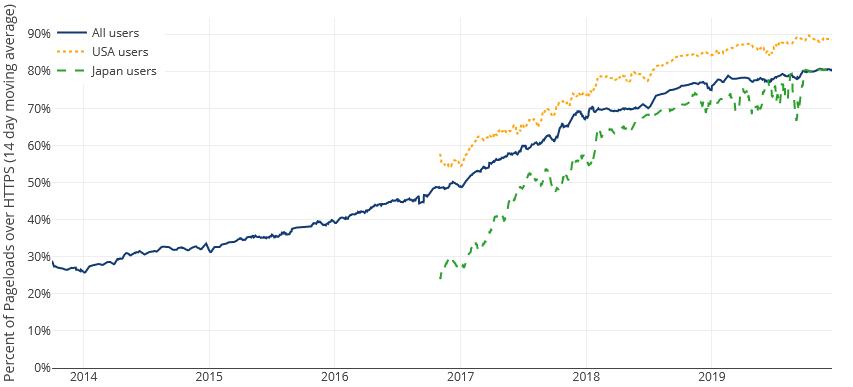
\includegraphics[width=0.8\textwidth]{ressources/https_statistics.png}
	\caption{Percentage of Web Pages Loaded by Firefox Using HTTPS \parencite{letsencrypt_lets_2019}}
\end{figure}

This could come due to several reasons. Whistleblower Edward Snowden has received a lot of media interest and has made people aware of using secure services on the Internet, when he revealed the capabilities of the National Security Agency (NSA). In addition, browser manufacturers like Mozilla or Google warn their users when they visit a website without HTTPS with an open red lock next to the address bar.
% Quelle NSA Snowden, http = unsecure google


\section{Motivation}

The use of public/private keys is too troublesome for many people, even IT professionals. The manual distribution of keys between several devices becomes more difficult the more devices there are. However, end-to-end encryption is only possible if multiple devices have the access to the same private key. The synchronization of private keys is often done via cloud providers, although they are also often attacked. The keys would either have to be additionally encrypted, which makes handling more difficult again, or distributed in another way. On the other hand, systems such as Android or iOS offer more and more security features in their latest versions, such as the generation of random numbers in their own encapsulated processor. It is therefore worth investigating to what extent this can be used to simplify the handling of private keys.

The use of public/private keys is too difficult for many people, even IT professionals. The keys have to be distributed and stored securely. In many cases the distribution of keys is done by synchronizing the keys within a cloud. However, this is a potential security leak, because cloud service providers are not entirely trustworthy. On the other hand, distributing private keys by universal serial bus (USB) is too time-consuming for many users. 

% \subsection{Entrepreneurial perspective}

% The adorsys GmbH \& Co. KG is a software development and consulting company that specializes in the fields of banking and insurance, but also develops software for industry companies. That's why internal security is especially important for adorsys and therefor also the security of communication within the company. Employees usually also have a smartphone that accesses corporate services. The management of key pairs, for example for secure email communication, is very important. 

% \subsection{Social perspective}

% The principles of private/public keys are 
% Secure email communication is also a rarity in the private environment. Even signatures, the certainty that the person who sent me the email is really who he claims to be, is usually not given. 
% One reason for this is that email communication was never developed to be secure. On the other hand, the key management and use for many is far too cumbersome. 

\section{Objective}

The goal of this work is to use a smartphone as a kind of secure wallet to store private keys on it. The private keys should never leave the smartphone. However, the smartphone must make the services of the private keys available to other applications, such as an email client on a desktop computer, so that encrypted emails can be read from there.

\section{Environment}

The work was carried out in cooperation with adorsys GmbH \& Co. KG. Founded in 2006, adorsys primarily offers software services in the banking and insurance industries. Adorsys became particularly well known through the open source implementation of the PSD2 payment directive, which came into force in 2019. The largest customers include Teambank AG, Datev eG, Bankverlag and ERGO Direkt. Adorsys has thus built up expertise in the financial sector, where security plays a major role. 

\section{Structural Overview}

%% Was passiert in den einzelnen Kapiteln

\chapter{Approach}

%% Wie bin ich in den einzelnen Kapiteln vorgegangen.
\section{Analysis of the current situation}

First of all, it is necessary to examine how keys are currently handled and their most common uses, where the end user needs to be able to access the keys. Use cases like the Diffie-Hellman should be excluded. 

\section{Requirements for Key-Distribution Systems}

After the frequent use cases have been identified, an analysis can be made of the requirements they place on key management. 

\section{Concept}

From the results of the requirements, a concept can be worked out how different systems can work together to best meet the requirements and provide the user with the best possible user experience. 

\section{Implementation}

With the help of the concept, a prototype can then be developed in the Implementation chapter, which fulfills the main functions of the concept in an exemplary manner. The findings that become visible during the development of the prototype can then be used to further improve the result of the work.


\chapter{Fundamentals}

\section{Quick-Response Codes}

Quick Response Codes (QR-Codes) are a kind of further development of barcodes, as they can be found on many products. Compared to barcodes, QR codes offer two dimensions instead of just one, which enables readers to read the codes faster and more robustly from different perspectives, but also contain more data. When a QR Code reader starts to analyze the code, it first calculates the ratio between the dark and light areas and then eliminates any possible distortion. Then the modules can be viewed, holding data ready to be used again. \parencite{office_masahiro_1994}

\section{Certificate Authority}
\label{sec:CA}

A Certificate Authority (CA) is an organization that creates digital certificates. The CA establishes a connection between a person or an organization and a public key. To create this connection, the CA must be able to check and confirm the identity of the person/organization. The public key is then signed, which allows other entities that trust the CA to be sure that it is the specified person/organization.
\parencite{luber_ca_2018}

\section{Certificate Signing Request}
\label{sec:CSR}

To have a certificate signed where a key pair already exists, a Certificate Signing Request (CSR) can be created. The advantage is that the private key does not have to be transferred to a CA but can remain secret. To do this, the customer must create a CSR to which information such as the common name (CN) is added. The CSR can then be signed with the customer's private key and sent to a CA to be signed. The CA then creates a digital certificate that the customer can distribute to communication partners.
\parencite{publico_ssl-grundlagen_2017}

%\section{Phishing}

\section{S/MIME}
Secure/Multipurpose Internet Mail Extensions (S/MIME) is one of the two main ways, how mail encryption can be accomplished. It is based on public-key cryptography. S/MIME can also be used to sign mails in order to clearly identify the sender of the message and also ensures, that the messages has not been manipulated, 
else this is easily possible and has already led to great damage through phishing attacks in the past. 
However, if the mail is only signed instead of encrypted, it can still be read by anyone who receives the data. \parencite{villadiego_dangers_2017}

S/MIME can also be classified into four different classes. The higher the class, the more certain the recipient can be that it is really the person in question.
\begin{itemize}
    \item Class 1: The CA only assures the authenticity of the mail address.
    \item Class 2: In addition to class 1, the name of the person and, if applicable, the company
    \item Class 3: Data provided from class 2 are confirmed by official documents.
    \item Class 4: Applicants must be physically present when the application is submitted
\end{itemize}

SMIME certificates can be signed by multiple Certificate Authorities. There are two possibilities for signing the keys. The first is that a Certification Authority gets the order to generate a new key pair, then sign it, hand it over to the customer and delete the keys (especially the private key) after completion. However, the customer cannot verify that the private key has been deleted or has not been copied before, so he cannot be sure that only he is in possession of the private key. The other possibility is to generate the keys locally and create a Certificate Signing Request as explained in section \ref{sec:CSR}.
\parencite{luber_smime_2018}

According to the principle of public-key cryptography, the private key of a user is used for signing and decrypting and the public key for encrypting and verifying a message.


\section{Elliptic Curve Cryptography}

Elliptical curve cryptography (ECC) is also based on the system of public-key cryptography. In comparison to other public-key cryptography systems such as RSA, algorithms that work with elliptic curves require a significantly smaller key length, which requires less computing power, but provide the same level of security. It can be used for creating and verifying signatures, but not for encryption. However, it can be combined with a Diffie-Hellman Key Exchange. In this way, encryption can also be implemented.
\parencite{hankerson_elliptic_2011}

\subsection{DH-Key Exchange using ECC}
The security is based on the fact that the addition of several points in a coordinate system is easy, but their division is much more difficult. To perform a key exchange, both parties must commit themselves to a predetermined elliptical curve and select a random point on it that intersects the curve. From this point, a tangent can then be constructed that intersects the curve at a new point. This point is then mirrored over the X axis and selected as the new starting point. Both parties repeat this procedure very often. The number of passes is then used as a private key. The resulting point (with its x and y values) is the public key that can be transmitted to the communication partner. Afterwards both parties repeat the calculation of the tangents and the corresponding points with the number of passes of their private key. Finally, both should come to the same end point, which is then the shared secret.
\parencite{hankerson_elliptic_2011}
% Vielleicht eine andere Quelle 
\begin{figure}[ht]
 \centering
 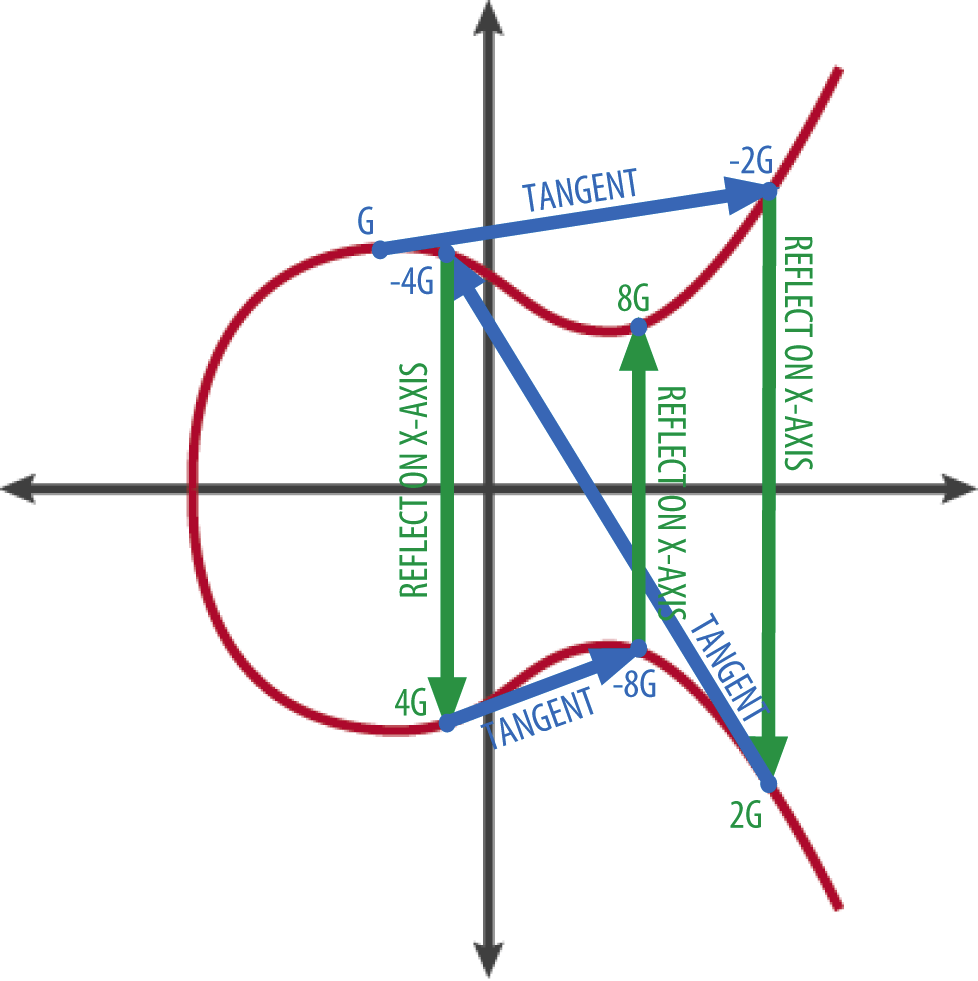
\includegraphics[width=0.8\textwidth]{ressources/ecc.png}
 \caption{Elliptic Curve Key Generation \parencite{uszak_elliptic_2017}}
 \label{fig:ecc}
\end{figure}

However, there are concerns that a back door has been built into one of the random number generators, on a curve which was created by the NSA (NIST-P256). Other curves that are not based on this are considered secure. 
\parencite{schneier_essays_2007}

% Vielleicht dass NIST-P-256 schlecht ist in die eigentliche Arbeit 

% \section{Secret Sharing}
\newpage
\section{ARM TrustZone}
\label{arm:TrustZone}

The ARM-TrustZone is an implementation for a Trusted Execution Environment (TEE) for ARM-Cortex based processors, which is the standard for mobile phones. It is a technology, which creates two environments, a trusted and a non-trusted, simultaneously on a single core. In each of the environments an own operating system is running. Software can run either in the trusted environment or the non-trusted. However, both environments can work together. For example an application running in the non-trusted enviroment can use a library which is running in the trusted environment. So, the TrustZone allows the secure storage of sensitive information like biometric information or Digital Rights Management (DRM) material, even if applications in the non-trusted environment are compromised.
\parencite{fowler_trustzone_2017}

\section{Hardware Security Module}
\label{sec:HSM}

A Hardware Security Module (HSM) is a peripheral device which, depending on the model, performs cryptographic functions for another computer system. This may include: Securely generating or managing cryptographic keys, protecting signatures and identities or establishing secure communication channels. It is important to note that the system using the functions of the module has no influence on the module, but can only call the functions. Such modules range from small USB tokens, such as the Ledger Nano S for crypto currency storage, to stand-alone servers that perform these cryptographic functions for a complete data center and are in addition certified for e.g. GDPR or HIPAA. As the name suggests, an HSM has separate hardware, as opposed to a Trusted Execution Environment as implemented by the ARM TrustZone. This usually consists of a CPU, separated secure storage and a generator for random numbers.
\parencite{sustek_hardware_2011}
% \parencite{ibm_hardware_2020} \parencite{gemalto_safenet_2020} 
% \section{Secure Element}

\section{Android Keystore System}

The Android keystore is a secure environment that is used to store keys and prevent their extraction as much as possible. To prevent extraction, the Android keystore follows several paths. Firstly, it gives the possibility to link the key to a secure hardware element if it supports the key type. Then the actual application never has full access to the generated key. If the application wants to perform cryptographic operations like signing, encrypting or decrypting, this does not happen inside the application, but the application requests the keystore to perform the requested operation. The keystore can also be used to specify exactly which applications should have access to the keystore. So if an app is compromised, the attacker can only perform the same operations as the user did before. For example, if an attack has taken place and countermeasures have been taken, it is ensured that the attacker cannot do operations with the key anymore. 
\parencite{google_android_2020}

\subsection{Hardware Backed Keystore}
\label{android:HWB}

With the different Generations of Android Versions, the Keystore System also has evolved. While Smartphones certified for Android Versions prior 'Marshmallow' (Android Version 6.0) only supported the creation of signatures, verification and generating/importing of asymmetric keys, newer versions (> Android 6.0) also support the usage of symmetric keys. Additionally, keys can be generated with hardware support, if the devices has an \nameref{arm:TrustZone} builtin, which is the case if the device supports authentication with a fingerprint or has access to DRM related material. If this is the case, the keystore is operating in a trusted environment and thus also performing cryptographic operations in it.
\parencite{google_hardware-backed_2020}
% Quelle für Fingerprint 


\subsection{Strongbox Keystore}

As an extension to the \nameref{android:HWB}, Google introduced a new security feature in Android Pie (Android Version 9.0), the StrongBox Keystore. The addition is, that the kind of Keystore implementation is specified by Google. With the \ref{android:HWB} every mobile phone manufacturer can implement their own TrustZone. Also, the StrongBox must operate on separated hardware to fulfill the specifications of a \nameref{sec:HSM} and to increase the security level by using dedicated hardware.

%% HW-Backed = various implementations like TrustZone
%% StrongBox = separated hardware

\section{iOS Keychain}

The iOS Keychain helps developers and users to store passwords or other sensible information. But also Keys, or things like certificates. There is also a built-in password manager that is designed for the user. The way it works is, that a secret which has to be stored gets packaged in a keychain item. Additionally, there should be packaged public attributes like a name or an identifier to make the item searchable. 

\begin{figure}[ht]
  \centering
  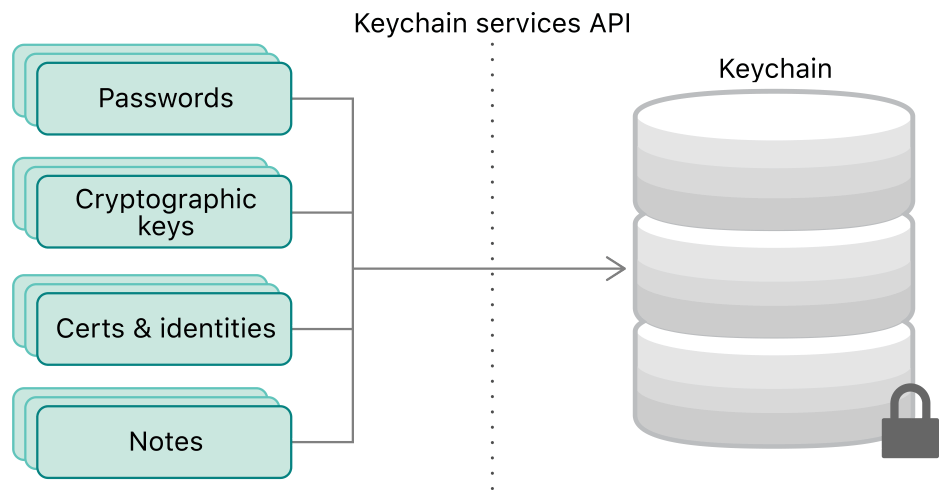
\includegraphics[width=0.8\textwidth]{ressources/apple_keychain.png}
  \caption{Apple Keychain \parencite{apple_keychain_2020}}
  \label{apple:keychain}
\end{figure}

It is an encrypted file in which all information that is particularly worth protecting is stored. In addition, this file can be synchronized via iCloud, Apple's cloud service, to make it available on all devices of a user. Particularly for the iPhone, every App can create its own keychain. Access to the Keychain can be additionally secured by authentication methods like FaceId or TouchId.

However, this means that the key was handled to some point in plaintext in the phone's memory, which could lead to a compromised key, if the app is also compromised. Apple created the Secure Enclave, which is a coprocessor doing cryptographic operations. This way the key never leaves the Secure Enclave and makes it harder for an adversary to compromise the key.
Apple has implemented this feature for all smartphones with an A7 processor chip or higher.
\parencite{apple_keychain_2020}

% \subsection{Common Crypto}

\subsection{iOS Secure Enclave}

Alike the \nameref{android:HWB}, the Secure Enclave is a coprocessor, which runs cryptographic operations. In addition, it is in possession of an own random-number generator, memory, operating-system and an encrypted storage. Thus, it can securely store keys, even if the kernel of the smartphone has been compromised. Also, cryptographic keys are never exposed to applications or the operating system of the main processor.
\parencite{apple_storing_2020} 

\subsection{Apple CryptoKit}

Since Version 13.0, Apple introduced a new cryptographic API for developers, the CryptoKit. The intention behind this is to simplify the use of cryptographic functions for developers. The most important functions are the generation and comparison of secure digests, public-key cryptography for digital signatures, as well as the execution of DH key exchange and the generation and use of symmetric keys. Also, it is possible to use private keys which are managed and generated by the Secure Enclave.

% \subsection{Security Framework}

% available from iOS 13+ upwards

% secure digest

% uses secure enclave in background

\newpage
\section{Signal-Protocol}

The signal protocol was developed by the Open Whisper Systems Foundation for their own messenger service Signal. It is an open standard end-to-end encryption protocol. The mayor benefit compared to other end-to-end encryption protocols is that messages can be sent encrypted even if the recipient is not online. This was also the reason for other messenger services such as WhatsApp, Skype or Facebook Messenger to implement a customized version of this encryption. 
\parencite{protocol_introducing_2018}



%\parencite{cohn-gordon_formal_2017}
% Quelle dafür das andere das auch eingebaut haben.


% Seitenzahl benoetigt wenn die komplette Arbeit daraus besteht?

\subsection*{Key Distribution Center}
\label{subsec:KDC}

In the Signal App, the Key Distribution Center exists to allow users to upload a bunch of keybundles so that they can be used by other users. In addition, messages that cannot be delivered at this point, because e.g. the receiver mobile phone is switched off, are stored there temporarily until they can be sent.

\subsection{Key Agreement Protocol - Extended Triple Diffie-Hellman}
The Key Agreement Protocol knows three parties. Alice, who would like to talk to Bob, Bob who wants other parties like Alice allow communicating with him and a server, which acts as the \nameref{subsec:KDC}. The keys needed for this key exchange are as follows:
\begin{itemize}
  \item Alice's identity key $   (IK_{A})  $
  \item Alice's ephemeral key $   ({EK_{A}})  $
  \item Bob's identity key $   ({IK_{B}})  $ 
  \item Bob's one-time prekey $   ({OPK_{B}})  $
\end{itemize}

Each of these keys is a key pair generated using elliptic curves (X25519 or X448). Though each of Bob's one-time prekeys can only be used once and Alice's ephemeral key is generated anew in each key exchange run.

The Key Agreement Protocol is build upon the Diffie-Hellman (DH) Key Exchange Protocol. However, the Extended Triple Diffie-Hellman (X3DH) is using three phases of the Key Agreement:
\begin{itemize}
  \item Bob uploads his identity key and several prekey bundles to a server.
  \item Alice requests one prekey bundle of Bob from the server.
  \item Bob receives a message from Alice and processes it.
\end{itemize}

After Alice receives the prekey bundle from the server, she checks the signature of the prekey. In the case that the signatures do not match, the protocol is aborted.
Otherwise, she generates an ephemeral key pair by using her own public key. Using this ephemeral key she can calculate a shared key (SK). After calculating the SK, she deletes the private ephemeral key and the DH outputs. Eventually, she calculates an associated data byte sequence which contains the identity keys of herself and Bob.
Finally, she can generate a message containing following keys:
\begin{itemize}
  \item Alice's identity key $    (IK_{A})  $
  \item Alice's ephemeral key $   {EK_{A}}  $
  \item An identifier which of the prekeys Alice used
  \item An initial ciphertext encrypted by the calculated shared key.
\end{itemize}

By receiving the message, Bob tries to decrypt the ciphertext by loading his identity key and the used prekey with the identifier send from Alice. With this information, Bob can repeat the calculations which were done by Alice and check if the results match and deletes the DH outputs. If not, he deletes everything he received and aborts the communication. If it was successful, he also deletes the used prekey for forward secrecy and can then use the SK for further encryption/decryption. 
\parencite{marlinspike_x3dh_2016}

\subsection{Double Ratcheting Algorithm}

The Double Ratchet Algorithm as used in the Signal-Protocol is a Key Derivation Function (KDF) algorithm, which is used to exchange encrypted messages by using a previously known SK. This SK can be generated by using some sort Key Exchange e.g. 3XDH, but outside this scope also by every other Key Exchange. As illustrated in the figure of the \nameref{fig:ratchet}, the KDF can only produce keys for other following steps, but not previous steps.

\begin{figure}[ht]
	\centering
  \includegraphics[width=0.8\textwidth]{ressources/ratchet.png}
  \caption{Mechanical Ratchet \parencite{pawl_rachet_2020}}
  \label{fig:ratchet}
\end{figure}
%Quelle für Bild (Wikimedia)

By using this algorithm, the generated keys would rather seem random to an adversary, if he doesn't know about the KDF-keys. Also, if gets in possession of one of the KDF-keys, older and future keys would also appear random to him. Using this algorithm, three different key chains are in use. A root chain, a transmitter and a corresponding receiver chain, which are the same on the opposing sides (Alice receiver chain is the same as Bob´s transmitter chain and vice versa). Also, the corresponding chains have to start at the same point and have to be synchronized. Figure \ref{fig:KDF_Chain} shows, how the chains are generating keys. The output key can be used to encrypt data, the KDF-key is used to calculate the next chain element.
\parencite{perrin_double_2016}

\begin{figure}[ht]
	\centering
  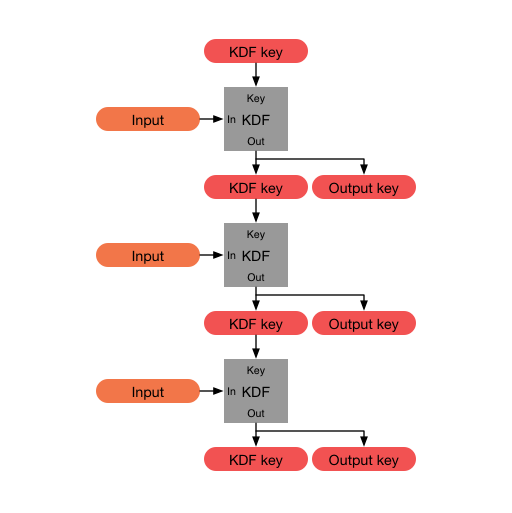
\includegraphics[width=0.8\textwidth]{ressources/kdf_chain.png}
  \caption{KDF Chain \parencite{perrin_double_2016}}
  \label{fig:KDF_Chain}
\end{figure}
\newpage

\subsubsection{Symmetric-key ratchet}

With the Symmetric-key ratchet, each message is encrypted with a unique message key. The message keys are generated with every ratchet step. In addition, a chain key is generated, which then can be is used as a KDF key for the ratchet step. The input, which can also be seen in figure \ref{fig:KDF_Chain}, is always a constant in the Symmetric-Key Ratchet, which means that if an attacker comes into possession of a chain key and the constant, he can decrypt subsequent messages. The message keys only ensure that each message is encrypted with a unique key and can theoretically be deleted after receiving the message. In addition, however, the respective keys contain a counter that allows the matching key to be found for the message, which could by possibility not arrive in the order, in which they were sent. Though, there is no security flaw in storing these message keys, because they are not used to generate other keys.
\parencite{perrin_double_2016}

\subsubsection{Diffie-Hellman ratchet}

If an adversary could steal the transmitter and receiver chain keys, it would be possible for him to decrypt all messages in the future. To prevent this from happening, the Double Ratcheting Algorithm combines two different types of KDF chains. While the transmitter and receiver chains are based on symmetric keychains, the root chain is a DH ratchet. The transmitter and receiver chains both use a DH-keypair from the root chain as starting point. With each message the Symmetric-key ratchet are extended by one chain link. However, to ensure security for messages in the future, the symmetric keychains' actually constant values are updated with the values from the DH ratchet, causing them to be reset. The root chain can always create new transmitter and receiver chains with new public keys. In the default implementation this happens with every message.
\parencite{perrin_double_2016}

%\chapter{Problem definition}

\chapter{Analysis of the current situation}

When designing a new type of key management, it is important to look at the current solutions and their characteristics. This helps to have a better overview of the functions required in the concept. In addition, the concept should also provide a way to make it as easy as possible for the user to use his keys on several devices and at the same time to have a simple administration of them. On the other hand, this step is also necessary to identify the problems of previous solutions so that they can be addressed in the concept. In a subsequent evaluation, the best solution in terms of security, usability and the required trust in third party providers can then be evaluated in various categories.

\section{Use Cases for distributed Keys}

\subsection{Email}

\subsection{SSH}
% Git und die eigentlichen VPN Verbindungen

\subsection{Password Manager}

\subsection{Two Factor Authentication}

\subsection{Crypto Currencies}

\subsection{VPN}



\section{Distribution of private keys}

\subsection{Local/Offline}

USB or some other offline connections are used to transfer the private key.

% \subsubsection{Subkeys}

% Only possible for pgp
% Only the latest subkey can be used to encrypt messages. Thus, every device must be in possession of this subkey. 

\subsection{Webservers/Downloads}

Possible vulnerability by man in the middle attacks.
The private key is stored on a trusted server. Whenever a new device is added, the user can download his private key.

\subsection{External Providers}

Using Services like Dropbox or Google drive. This can be combined with encrypting the private key and or separating the key using secret sharing and 
storing them on different clouds. 




\chapter{Requirements for Key-Distribution Systems}

\section{Usability}

\section{Security}

Enter a passphrase on computer and then on mobile phone would add security but isn't that convenient.

%\section{Loss Coverage}
% Kommt nur in ausblick
\chapter{Concept}

\section{Architecture}

\section{Usability}

\chapter{Implementation}

\section{Kotlin}

\section{gRPC}

\section{Prototype}

\subsection{App}

\subsection{Desktop Client}

% Nach dem verbinden mit QR Code könnte in der App eine Pin angezeigt werden die dann am PC eingegeben werden muss.


\chapter{Evaluation}

\section{Usability}

\section{Security}

%\section{Existing Solutions}

%\section{QR-Based Solution}

\chapter{Summary}

\chapter{Outlook}

Backup can be implemented using social secret sharing or other things.

You could create clients for all kinds of desktop Programs, ssh, pgp, and so on.

\backmatter
%%%%%%%%%%%%%%%%%%%
%% create figure list
%%%%%%%%%%%%%%%%%%%

\listoffigures
\addcontentsline{toc}{chapter}{Directories}

%%%%%%%%%%%%%%%%%%%
%% create tables list
%%%%%%%%%%%%%%%%%%%
\listoftables

%%%%%%%%%%%%%%%%%%%
%% create listings list
%%%%%%%%%%%%%%%%%%%
%\lstlistoflistings
%\addcontentsline{toc}{chapter}{Listings}

\cleardoublepage
\phantomsection
\addcontentsline{toc}{chapter}{Bibliography}
\printbibliography

%%%%%%%%%%%%%%%%%%%
%% declaration on oath
%%%%%%%%%%%%%%%%%%%

\addchap{Affidavit}

I hereby certify that I have written my bachelor thesis independently and have not yet submitted it for examination purposes elsewhere. All sources and aids used are listed, literal and meaningful quotations have been marked as such.

\vspace{20pt}
\begin{flushright}
$\overline{~~~~~~~~~~~~~~~~~\mbox{\ShowBaAuthor, am \today}~~~~~~~~~~~~~~~~~}$
\end{flushright}

\addchap{Consent to plagiarism check}

I hereby agree that my submitted work may be sent to PlagScan (www.plagscan.com) in digital form for the purpose of checking for plagiarism and that it may be temporarily (max. 5~years) stored in the database maintained by PlagScan as well as personal data which are part of this work may be stored there.

\begin{small}
This Consent is voluntary. Without this consent, the plagiarism check can still take place, when all personal data is removed from the document. Consent to the storage and use of personal data may be revoked at any time by notifying the faculty.
\end{small}

\vspace{20pt}
\begin{flushright}
$\overline{~~~~~~~~~~~~~~~~~\mbox{\ShowBaAuthor, am \today}~~~~~~~~~~~~~~~~~}$
\end{flushright}

\end{document}
